
\subsection{Definicion del problema Subset Sum}
Dado un conjunto de n \'items $S$, cada uno con un $valor$ asociado $v_{i}$ , y un valor objetivo $V$ ,
decidir si existe un subconjunto de \'items de S que sumen exacto el valor objetivo $V$ . Si existe
dicho conjunto, decir cual es la m\'inima cardinalidad
P entre todos los subconjuntos posibles. \\
En otras palabras decidir si existe$ R \subseteq S$ tal que $\sum_{i \in R}v_{i} = V$, y si existe, devolver la menor cardinalidad posible de $R$.\\
Para este problema, asumiremos que todos los valores mencionados son enteros no negativos.
\subsection{Ejemplo de problema}

tomar el elemento(con un - arriba del nodo) para mirar si forma parte de la solución.
En este ejemplo se puede ver cual es el espacio de soluciones, la forma de recorrerlo será
definida más adelante  de acuerdo a cada algoritmo que usemos para resolver el problema.
Además se ver\'a que tamaño tiene este espacio, y la cantidad de posibles soluciones (en el diagrama trivialmente se logra ver como cada nodo hoja es una posible soluci\'on que llego desde las decisiones tomadas).
\subsubsection{Ejemplo 1}
En este ejemplo, se considera un conjunto de 4 elementos {11,7,5,2}.
Se busca que la suma de los elementos sea 18 y que el cardinal sea mínimo.
El nivel i representa la decisión de tomar el elemento(con un + arriba del nodo) o no
Como se puede ver en la imagen, hay dos soluciones {11,7} y {11,5,2} que suman 18 pero
la mejor es usando menos elementos, con lo cual nos quedamos con la solución {11,7}.
\begin{center}
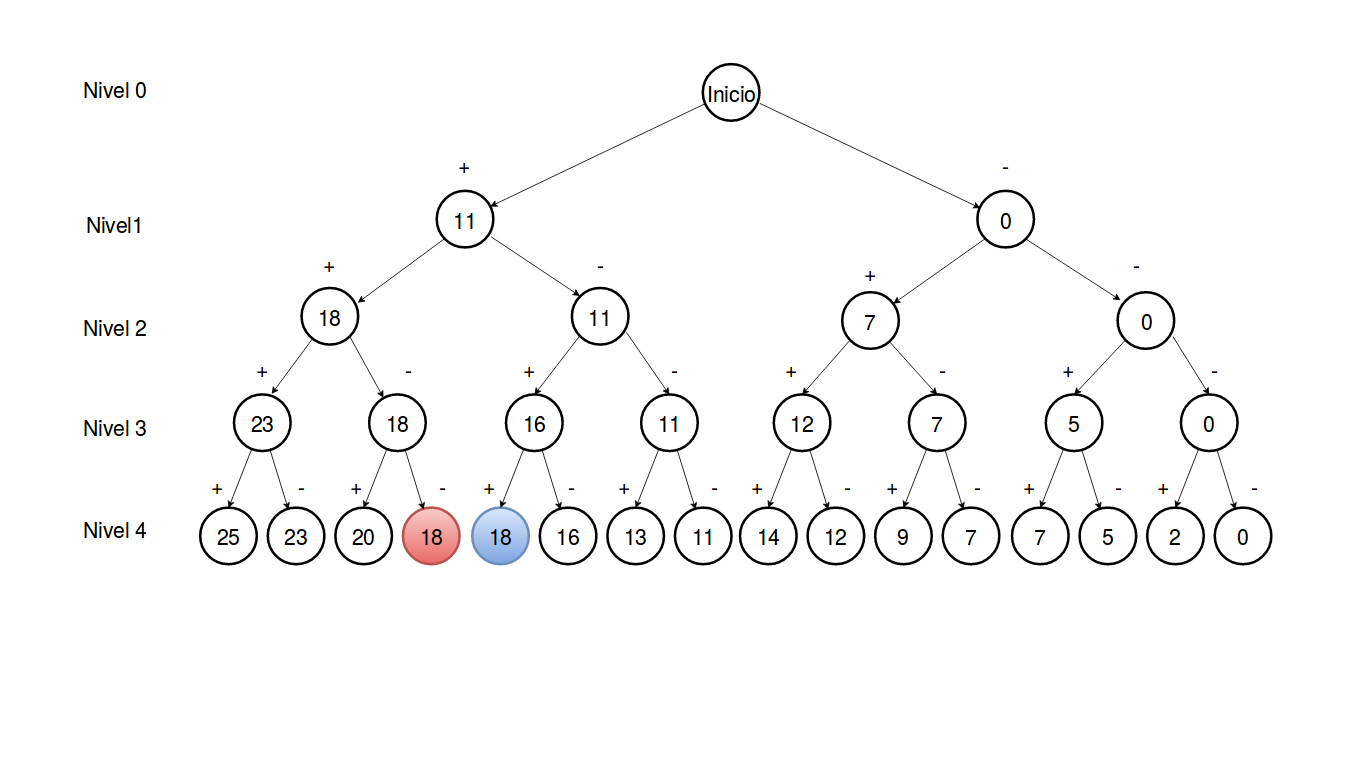
\includegraphics[width=18cm, height=12cm]{diagrama.png}
\end{center}
\newpage
\subsubsection{Ejemplo 2}
Conjunto $\{2, 3, 12, 14, 4\}$, buscamos un subconjunto de elementos que sume 13.\\
El 14, no puede sumar 13. El 12 no se puede elegir porque no hay elementos que sumen 1. Al combinar cualquiera de los que restan, no alcanzan a sumar 13 con lo cual no hay soluci\'on para este problema.\\


\subsection{El objetivo del trabajo practico}
 Resolver el problema propuesto de diferentes maneras realizando posteriormente una comparaci\'on entre los diferentes algoritmos utilizados.